%
% Flächenintegrale
%
\section{Flächenintegrale von 2-Formen
\label{buch:green:section:integral}}
In Abschnitt~\ref{buch:kurvenintegral:section:1form} wurde gezeigt,
wie das Integral einer 1-Form entlang einer Kurve als
koordinatensystemunabhängige Grösse definiert werden kann.
Entscheidend war die Erkenntnis, dass das Integral der Werte einer
Funktion entlang der Kurve von der Parametrisierung, also dem
Koordinatensystem, der Kurve abhängt.
Nur eine 1-Form hat das richtige Transformationsverhalten beim
Wechsel des Koordinatensystems, das zu einer koordinatensystemunabhängigen
Definition führt.
In diesem Abschnitt wird diese Überlegung auf zweifache Integrale
verallgemeinert.

\kopfrechts{Flächenintegrale}%

%
% Integral einer 2-Form auf R^2
%
\subsection{Integral einer 2-Form auf $\mathbb{R}^2$}
Wir betrachten eine differenzierbare Funktion
$f\colon \mathbb{R}^2\to\mathbb{R}$ zweier Variablen.
Zusätzlich sei angenommen, dass $f$ kompakten Träger hat. 
Dann ist dass Integral von $f$ über $\mathbb{R}^2$ wohldefiniert
und kann mit Hilfe des Satzes von Fubini als iteriertes Integral
\index{Satz!von Fubini}%
\begin{equation}
\int_{\mathbb{R}^2} f(x^1,x^2)\,dx^1\,dx^2
=
\int_{\mathbb{R}} \biggl(\int_{\mathbb{R}} f(x^1,x^2) \,dx^1\biggr) \,dx^2
=
\int_{\mathbb{R}} \biggl(\int_{\mathbb{R}} f(x^1,x^2) \,dx^2\biggr) \,dx^1
\label{buch:green:flaechenintegral:eqn:int2}
\end{equation}
berechnet werden.
Die Klammern sind nur zur Verdeutlichung der möglichen
unterschiedlichen Integrationsreihenfolgen.
Das innere Integral hängt von einem Parameter $x^2$ bzw.~$x^1$ ab.
Das Resultat dieser Integration ist daher eine differenzierbare
Funktion nur noch von $x^2$ bzw.~$x^1$, die wieder integrierbar ist.

Das Integral~\eqref{buch:green:flaechenintegral:eqn:int2} kann jedoch
nicht koordinatenunabhängig sein.
%
% fig-volint.tex
%
% (c) 2025 Prof Dr Andreas Müller
%
\begin{figure}
\centering
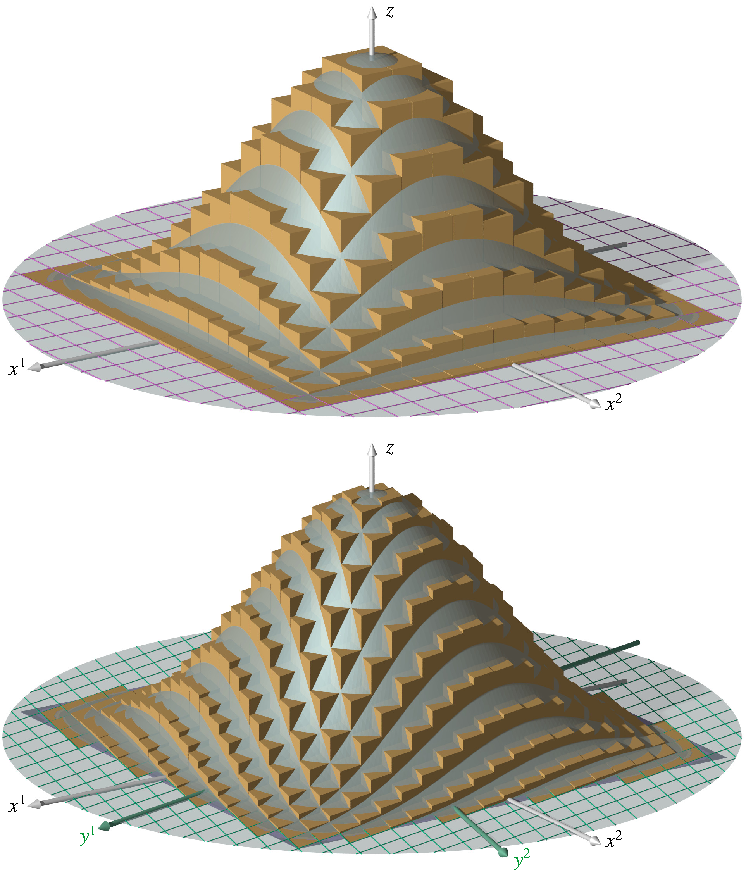
\includegraphics[width=\textwidth]{chapters/040-green/images/volint.pdf}
\caption{Volumen unter dem Graphen der Funktion $f(x^1,x^2)$ berechnet mit
zwei verschiedenen Parametrisierungen der Ebene.
In den $(x^1,x^2)$-Koordinaten wird das Volumen als Summe von Quadern
approximiert.
In den $(y^1,y^2)$-Koordinaten werden Prismen mit parallelogrammförmigen
Grundflächen aufaddiert.
Eine koordinatenunabhängige Grösse entsteht nur, wenn die Änderung
der Prismengrundfläche berücksichtigt wird.
\label{buch:green:fig:volint}}
\end{figure}
%
Dazu interpretieren wir das Integral als das Volumen unter einer der 
Fläche, die der Graph der Funkion $f(x^1,x^2)$ ist.
Es setzt sich approximativ zusammen aus kleinen Quadern mit
rechteckiger Grundfläche $\Delta x^1 \times \Delta x^2$ und Höhe
$f(x^1,x^2)$.
Das gleiche Volumen wird nach einer lineare Transformation 
\[
\begin{aligned}
x^1 &= a^1\mathstrut_1 y^1 + a^1\mathstrut_2 y^2 \\
x^2 &= a^2\mathstrut_1 y^1 + a^2\mathstrut_2 y^2 
\end{aligned}
\]
durch eine Summe von Prismen approximiert, die Höhe $f(y^1,y^2)$ haben,
\index{Prisma}%
aber als Grundfläche ein Parallelogramm, mit den Kantenvektoren
\[
\begin{pmatrix}
a^1\mathstrut_1\\
a^2\mathstrut_1
\end{pmatrix}
\Delta y^1
\qquad\text{und}\qquad
\begin{pmatrix}
a^1\mathstrut_2\\
a^2\mathstrut_2
\end{pmatrix}
\Delta y^2.
\]
Der Flächeneinhalt eines solchen Parallelogramms ist die Determinante
\[
F
=
\left|\,
\begin{matrix}
a^1\mathstrut_1 & a^1\mathstrut_2 \\
a^2\mathstrut_1 & a^2\mathstrut_2
\end{matrix}
\,\right|
\Delta y^1\cdot \Delta y^2.
\]
Um also das gleiche Volumen wie von
\eqref{buch:green:flaechenintegral:eqn:int2}
zu erhalten, muss das Integral
\[
\int_{\mathbb{R}^2}
f(x^1,x^2)
\,dx^1\,dx^2
=
\int_{\mathbb{R}^2}
f(y^1,y^2)
\left|\,
\begin{matrix}
a^1\mathstrut_1 & a^1\mathstrut_2 \\
a^2\mathstrut_1 & a^2\mathstrut_2
\end{matrix}
\,\right|
\,dy^1\,dy^2
\]
berechnet werden.
Die Verzerrung des Gitters ist in Abbildung~\ref{buch:green:fig:volint}
dargestellt.
Der Determinantenfaktor rechnet das Volumen des Einheitsquadrates in den
$(y^1,y^2)$-Koordinaten um in den Flächeninhalt des Grundseitenparallelogramms
eines Prismas in den $(x^1,x^2)$-Koordinaten.

Eine Funktion hat also nicht die richtigen Transformationseigenschaften.
Die Determinante
\[
\det A
=
a^1\mathstrut_1
a^2\mathstrut_2
-
a^1\mathstrut_2
a^2\mathstrut_1
\]
bedeutet, dass bei der Transformation des Integranden auf ein anderes
Koordinatensystem immer zwei Faktoren aus der
Transformationsmatrix auftauchen.
Bei einem Tensor erster Stufe ist dies nicht möglich.
Nur mit einem Tensor zweiter Stufe ist es möglich, solche Produkte 
in der Transformationsformel zu haben.

Seien also jetzt $f_{ik}$ die Koeffizienten eines Tensors 
\emph{zweiter Stufe} in $x$-Koordinaten und $\tilde{f}_{lm}$ die Koeffizienten
des Tensors in den $y$-Koordinaten.
Die Transformationsformel ist dann
\begin{align}
\tilde{f}_{lm}
&=
\sum_{i,k=1}^2
f_{ik}\, a^i\mathstrut_l\, a^k\mathstrut_m.
\intertext{Die Transformation soll nur die Determinante von $A$
hinzufügen.
Schreibt man die Transformationsformeln für den Tensor $f$ aus, erhält man}
\tilde{f}_{11}
&=
f_{11}\, a^1\mathstrut_1\, a^1\mathstrut_1
+
f_{12}\, a^1\mathstrut_1\, a^2\mathstrut_1
+
f_{21}\, a^2\mathstrut_1\, a^1\mathstrut_1
+
f_{22}\, a^2\mathstrut_1\, a^2\mathstrut_1
\\
\tilde{f}_{12}
&=
f_{11}\, a^1\mathstrut_1\, a^1\mathstrut_2
+
f_{12}\, a^1\mathstrut_1\, a^2\mathstrut_2
+
f_{21}\, a^2\mathstrut_1\, a^1\mathstrut_2
+
f_{22}\, a^2\mathstrut_1\, a^2\mathstrut_2
\\
\tilde{f}_{21}
&=
f_{11}\, a^1\mathstrut_2\, a^1\mathstrut_1
+
f_{12}\, a^1\mathstrut_2\, a^2\mathstrut_1
+
f_{21}\, a^2\mathstrut_2\, a^1\mathstrut_1
+
f_{22}\, a^2\mathstrut_2\, a^2\mathstrut_1
\\
\tilde{f}_{22}
&=
f_{11}\, a^1\mathstrut_2\, a^1\mathstrut_2
+
f_{12}\, a^1\mathstrut_2\, a^2\mathstrut_2
+
f_{21}\, a^2\mathstrut_2\, a^1\mathstrut_2
+
f_{22}\, a^2\mathstrut_2\, a^2\mathstrut_2.
\end{align}
Diese Formeln können nur dann ausschliesslich den Faktor $\det A$ ergeben,
wenn alle Terme verschwinden, in denen andere Produkte von $a^s\mathstrut_r$
als in der Determinante vorkommen.
Daraus kann man schliessen, dass $f_{11}=f_{12}=0$ sein muss.
Es bleiben  dann die Gleichungen
\begin{align*}
0
&=
f_{12}\, a^1\mathstrut_1\, a^2\mathstrut_1
+
f_{21}\, a^2\mathstrut_1\, a^1\mathstrut_1
=
(f_{12}+f_{21})\, a^1\mathstrut_1\, a^2\mathstrut_1
\\
\tilde{f}_{12}
&=
f_{12}\, a^1\mathstrut_1\, a^2\mathstrut_2
+
f_{21}\, a^2\mathstrut_1\, a^1\mathstrut_2
\\
\tilde{f}_{21}
&=
f_{12}\, a^1\mathstrut_2\, a^2\mathstrut_1
+
f_{21}\, a^2\mathstrut_2\, a^1\mathstrut_1
\\
0
&=
f_{12}\, a^1\mathstrut_2\, a^2\mathstrut_2
+
f_{21}\, a^2\mathstrut_2\, a^1\mathstrut_2
=
(f_{12}+f_{21}) a^1\mathstrut_2\, a^2\mathstrut_2
\end{align*}
Die erste und die letzte dieser Gleichungen können nur erfüllt sein,
wenn $f_{12}=-f_{21}$, $f$ muss also ein antisymmetrischer
Tensor sein.
Es bleiben dann nur noch die mittleren beiden Gleichungen,
die sich zu
\begin{align*}
\tilde{f}_{12}
&=
f_{12}\,(a^1\mathstrut_1\, a^2\mathstrut_2
-
a^2\mathstrut_1\, a^1\mathstrut_2)
=
f_{12}\,\det A
\\
\tilde{f}_{21}
&=
f_{12}\,(- a^1\mathstrut_2\, a^2\mathstrut_1
+
a^2\mathstrut_2\, a^1\mathstrut_1)
=
-f_{21}\,\det A
\end{align*}
vereinfachen.
Genau die antisymmetrischen kovarianten Tensoren haben also ein
koordinatensystemunabhängiges Integral.
Ein antisymmetrischer Tensor $f_{ik}$ zweiter Stufe auf $\mathbb{R}^2$
ist durch die einzige unabhängige Komponente $f_{12}$ bereits
festgelegt, weil $f_{11}=f_{22}=0$ und $f_{21}=-f_{12}$.

\begin{definition}
\label{buch:green:flaechenintegral:2formintegral}
Eine 2-Form auf $\mathbb{R}^2$ ist ein antisymmetrischer, kovarianter Tensor
\index{2-Form}%
\[
\omega
=
f_{12}\, dx^1\wedge dx^2
\]
zweiter Stufe.
Das Integral der 2-Form $\omega$ ist
\[
\int_{\mathbb{R}^2}
\omega
=
\int_{\mathbb{R}^2}
f_{12}\, dx^1\wedge dx^2
=
\int_{-\infty}^\infty
\int_{-\infty}^\infty
%\int_{\mathbb{R}^2}
f_{12}(x)
\,
dx^1\,dx^2.
\]
\end{definition}

%
% Kartenwechsel und Koordinatentransformation von 2-Formen
%
\subsection{Kartenwechsel und Koordinatentransformation von 2-Formen}
Eine 2-Form führt auf die richtigen Transformationsformeln für ein Integral.
In einem Koordinatengebiet kann daher das Integral durch die Formel
der Definition~\ref{buch:green:flaechenintegral:2formintegral}
berechnet werden.
Für eine 2-Form, deren Träger in einer Karte enthalten ist, ist
damit das Integral der 2-Form definiert.

In der Schnittmenge zweier Karten $(U_x,\varphi_x)$ und $(U_y,\varphi_y)$
gibt es zwei verschiedene Koordinatensysteme.
Die Kartenwechselabbildung $\varphi$ zwischen den beiden Karten ist
$\varphi=\varphi_x\circ\varphi_y^{-1}$, sie bildet $y$ auf
$x=\varphi(y)$ ab.
Falls die 2-Form $\omega$ Träger in der Schnittmenge der Karten hat,
kann das Integral auf zwei verschieden Arten berechnet werden,
die den gleichen Wert ergeben.
Auf den beiden Kartengebieten wird die 2-Form durch
\[
\omega
=
f_{12}(x)\,dx^1\wedge dx^2\quad\text{auf $\varphi_x(U_x)$}
\qquad\text{und}\qquad
\omega
=
\tilde{f}_{12}(y)\,dy^1\wedge dy^2\quad\text{auf $\varphi_y(U_y)$}
\]
gegeben.
Wir stellen uns die Funktionen $f_{12}(x)$ und $\tilde{f}_{12}(y)$
durch 0 auf ganz $\mathbb{R}^2$ fortgesetzt, damit wir uns nicht um
Integralgrenzen kümmern müssen.
Dann kann der Wert des Integrals von $\omega$ durch
\begin{equation}
\begin{aligned}
\int \omega
&=
\int_{U_x} f_{12}(x) \,dx^1\wedge dx^2
=
\int_{-\infty}^\infty\int_{-\infty}^\infty f_{12}(x)\,dx^1\,dx^2
\\
&=
\int_{U_y} \tilde{f}_{12}(y) \,dy^1\wedge dy^2
=
\int_{-\infty}^\infty\int_{-\infty}^\infty \tilde{f}_{12}(y)\,dy^1\,dy^2
\end{aligned}
\label{buch:green:flaechenintegral:eqn:2integrale}
\end{equation}
mit
\[
\tilde{f}_{12}(y)
=
f_{12}(\varphi(y))
\,
\left|
\frac{\partial(x^1,x^2)}{\partial(y^1,y^2)}
\right|
=
f_{12}(\varphi(y))
\,
\det(D\varphi(y))
\]
mit der Kartenwechselabbildung $\varphi=\varphi_x\circ\varphi_y^{-1}$
ergeben.

Wenn der Träger der 2-Form nicht in einer einzelnen Karte Platz
findet, dann muss die 2-Form in 2-Formen aufgeteilt werden, deren
Träger jeweils in einem Kartengebiet enthalten ist.
Im Abschnitt~\ref{buch:green:satzvongreen:subsection:zerlegung}
wird gezeigt, wie dies mit einer differenzierbaren Zerlegung
der Einheit erreicht werden kann.
Dies wird sicherstellen, dass einer 2-Form auf einer
zweidimensionalen Mannigfaltigkeit auch dann ein eindeutig bestimmter
Wert zugeordnet werden kann, wenn der Träger in keiner Karte Platz
findet.

%
% Orientierung einer 2-dimensionalen Mannigfaltigkeit
%
\subsection{Orientierung einer 2-dimensionalen Mannigfaltigkeit}
Kartenwechsel zwischen zwei Karten einer 2-dimensionalen
Mannigfaltigkeit sind differenzierbare und invertierbare Abbildungen
$f$ zwischen offenen Mengen von $\mathbb{R}^2$.
Die Ableitung $Df$ muss invertierbar sein.
Als lineare Abbildung ist das genau dann der Fall, wenn die Determinante
von $0$ verschieden ist.
In einem zusammenhängenden Gebiet muss daher die Determinante
von $Df$ überall das gleiche Vorzeichen haben.

Kartenwechsel zwischen zwei Karten einer 2-dimensionalen Mannigfaltigkeit
geben Anlass zu einer linearen Abbildung der 2-Formen.
Da der Vektorraum der 2-Formen aber eindimensional ist, ist diese
lineare Abbildung durch ein einzige Zahl gegeben, nämlich duch die
Determinante der Ableitung des Kartenwechsels.
Ein Kartenwechsel kann also das Vorzeichen des Koeffizienten
von $dx^1\wedge dx^2$ ändern oder gleich belassen.

\begin{beispiel}
\label{buch:green:green:beispiel:band}
%
% fig-band.tex
%
% (c) 2025 Prof Dr Andreas Müller
%
\begin{figure}
\centering
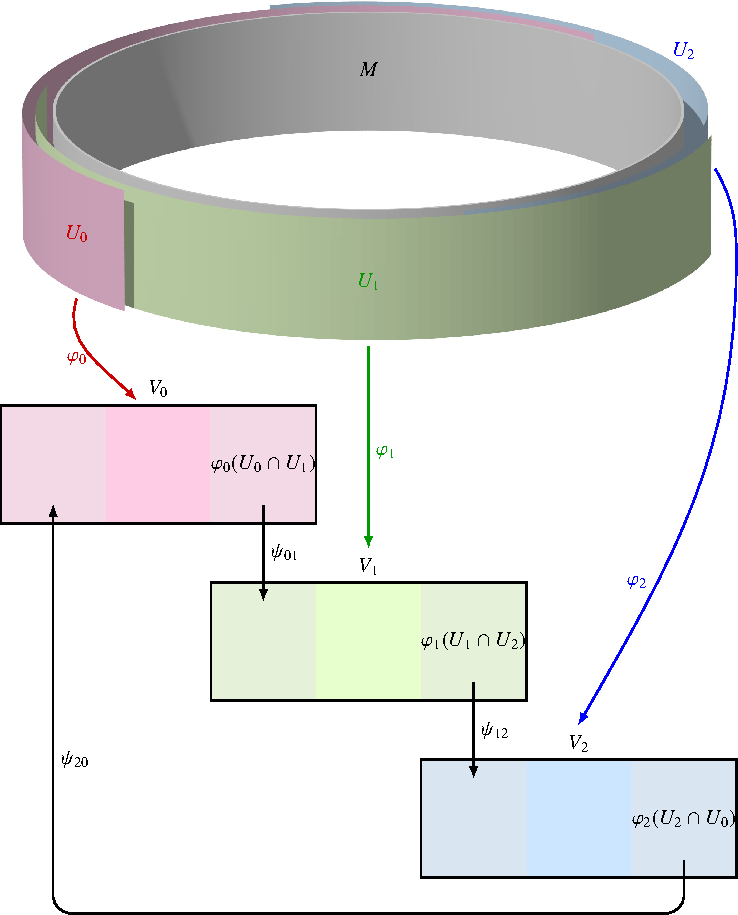
\includegraphics{chapters/040-green/images/band.pdf}
\caption{Zylindrisches Band mit drei Karten und drei Kartenwechselgebieten,
in denen die Determinante der Ableitung des Kartenwechsels positiv ist.
Das Band ist daher orientierbar.
\label{buch:green:green:fig:band}}
\end{figure}

Die Mannigfaltigkeit $M$ von Abbildung~\ref{buch:green:green:fig:band}
wird durch die drei Kartengebiete
\begin{align*}
V_0&=\psi_0(U_0) = \biggl(-\frac{\pi}3,\frac{5\pi}3\biggr)\times(-l,l),
\\
V_1&=\psi_1(U_1) = \biggl(-\frac{\pi}3,\frac{5\pi}3\biggr)\times(-l,l)
\\
\text{und}\qquad
V_2&=\psi_2(U_2) = \biggl(-\frac{\pi}3,\frac{5\pi}3\biggr)\times(-l,l)
\end{align*}
und die Kartenwechselabbildungen
\begin{align*}
\psi_{01}&\colon
\psi_0(U_0\cap U_1)
\to
V_1
:(x,y) \mapsto \biggl(x-\frac{2\pi}3,y\biggr)
\\
\psi_{12}&\colon
\psi_1(U_1\cap U_2)
\to
V_2
:(x,y) \mapsto \biggl(x-\frac{2\pi}3,y\biggr)
\\
\psi_{20}&\colon
\psi_2(U_2\cap U_0)
\to
V_0
:(x,y) \mapsto \biggl(x-\frac{2\pi}3,y\biggr)
\end{align*}
Die drei Kartengebiete sind Rechtecke.
Die Ableitung der Kartenwechselabbildung hat als Matrix die Einheitsmatrix,
die positive Determinante hat.
Auf dieser Mannigfaltigkeit gibt es eine 2-Form, die in jedem 
Kartengebiet durch $dx\wedge dy$ gegeben ist.
Insbesondere hat diese 2-Form keine Nullstellen.
\end{beispiel}


\begin{beispiel}
\label{buch:green:green:beispiel:moebius}
%
% fig-moebius.tex
%
% (c) 2025 Prof Dr Andreas Müller
%
\begin{figure}
\centering
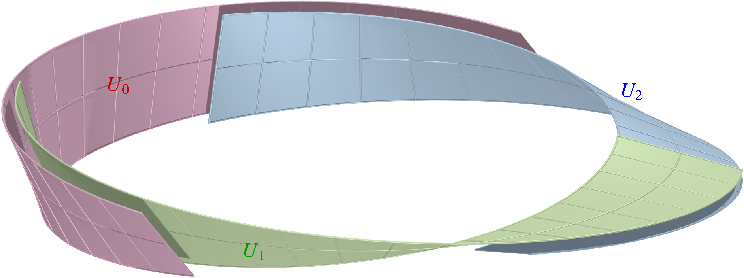
\includegraphics{chapters/040-green/images/moebius.pdf}
\caption{Durch Änderung einer einzigen Kartenwechselabbildung entsteht
ein Atlas für ein Möbius-Band, welches nicht orientierbar ist.
\label{buch:green:green:fig:moebius}}
\end{figure}
%
Durch Änderung der Kartenwechselabbildung $\psi_{12}$ in
\begin{align*}
\psi_{12}&\colon
\psi_1(U_1\cap U_2)
\to
V_2
:(x,y) \mapsto \biggl(x-\frac{2\pi}3,-y\biggr)
\end{align*}
entsteht ein neuer Atlas, der aber nicht mehr ein zylindrisches Band
beschreibt.
In Abbildung~\ref{buch:green:green:fig:moebius} wird das gemeinsame
Gebiet $U_1\cap U_2$ der grünen und der blauen Karte gespiegelt,
was einem um $180^\circ$ verdrehten Band entspricht.
Dies ein Möbius-Band.

Auf dem Möbius-Band gibt es keine 2-Form ohne Nullstellen.
\index{Mobius-Band@Möbius-Band}%
Gäbe es eine solche 2-Form $\omega$, dann könnten wir die Komponenten
in der roten und der grünen Karte $U_0$ und $U_1$ so ändern, dass
$\omega$ auf beiden durch $dx\wedge dy$ gegeben ist.
Dann muss nur noch eine Darstellung $u(x,y)\,dx\wedge dy$ für die 
blaue Karte $U_2$ gefunden werden.
Auf dem Überschneidungsgebiet $\varphi_2(U_0\cap U_2)$ muss $u(x,y)=1$
sein.
Auf dem Überschneidungsgebiet $\varphi_2(U_1\cap U_2)$ ist die 
Determinante des Kartenwechsels $-1$, d.~h.~dort muss $u(x,y)=-1$
sein.
$u(x,y)$ ist daher eine differenzierbare Funktion auf dem zusammenhängend
Rechteck $V_2$, welche am einen Ende den Wert $1$ und am anderen den 
Wert $-1$ haben muss.
Nach dem Zwischenwertsatz muss diese Funktion eine Nullstelle haben,
im Widerspruch zur Annahme.
\end{beispiel}

%
% fig-ants.tex
%
% (c) 2025 Prof Dr Andreas Müller
%
\begin{figure}
\centering
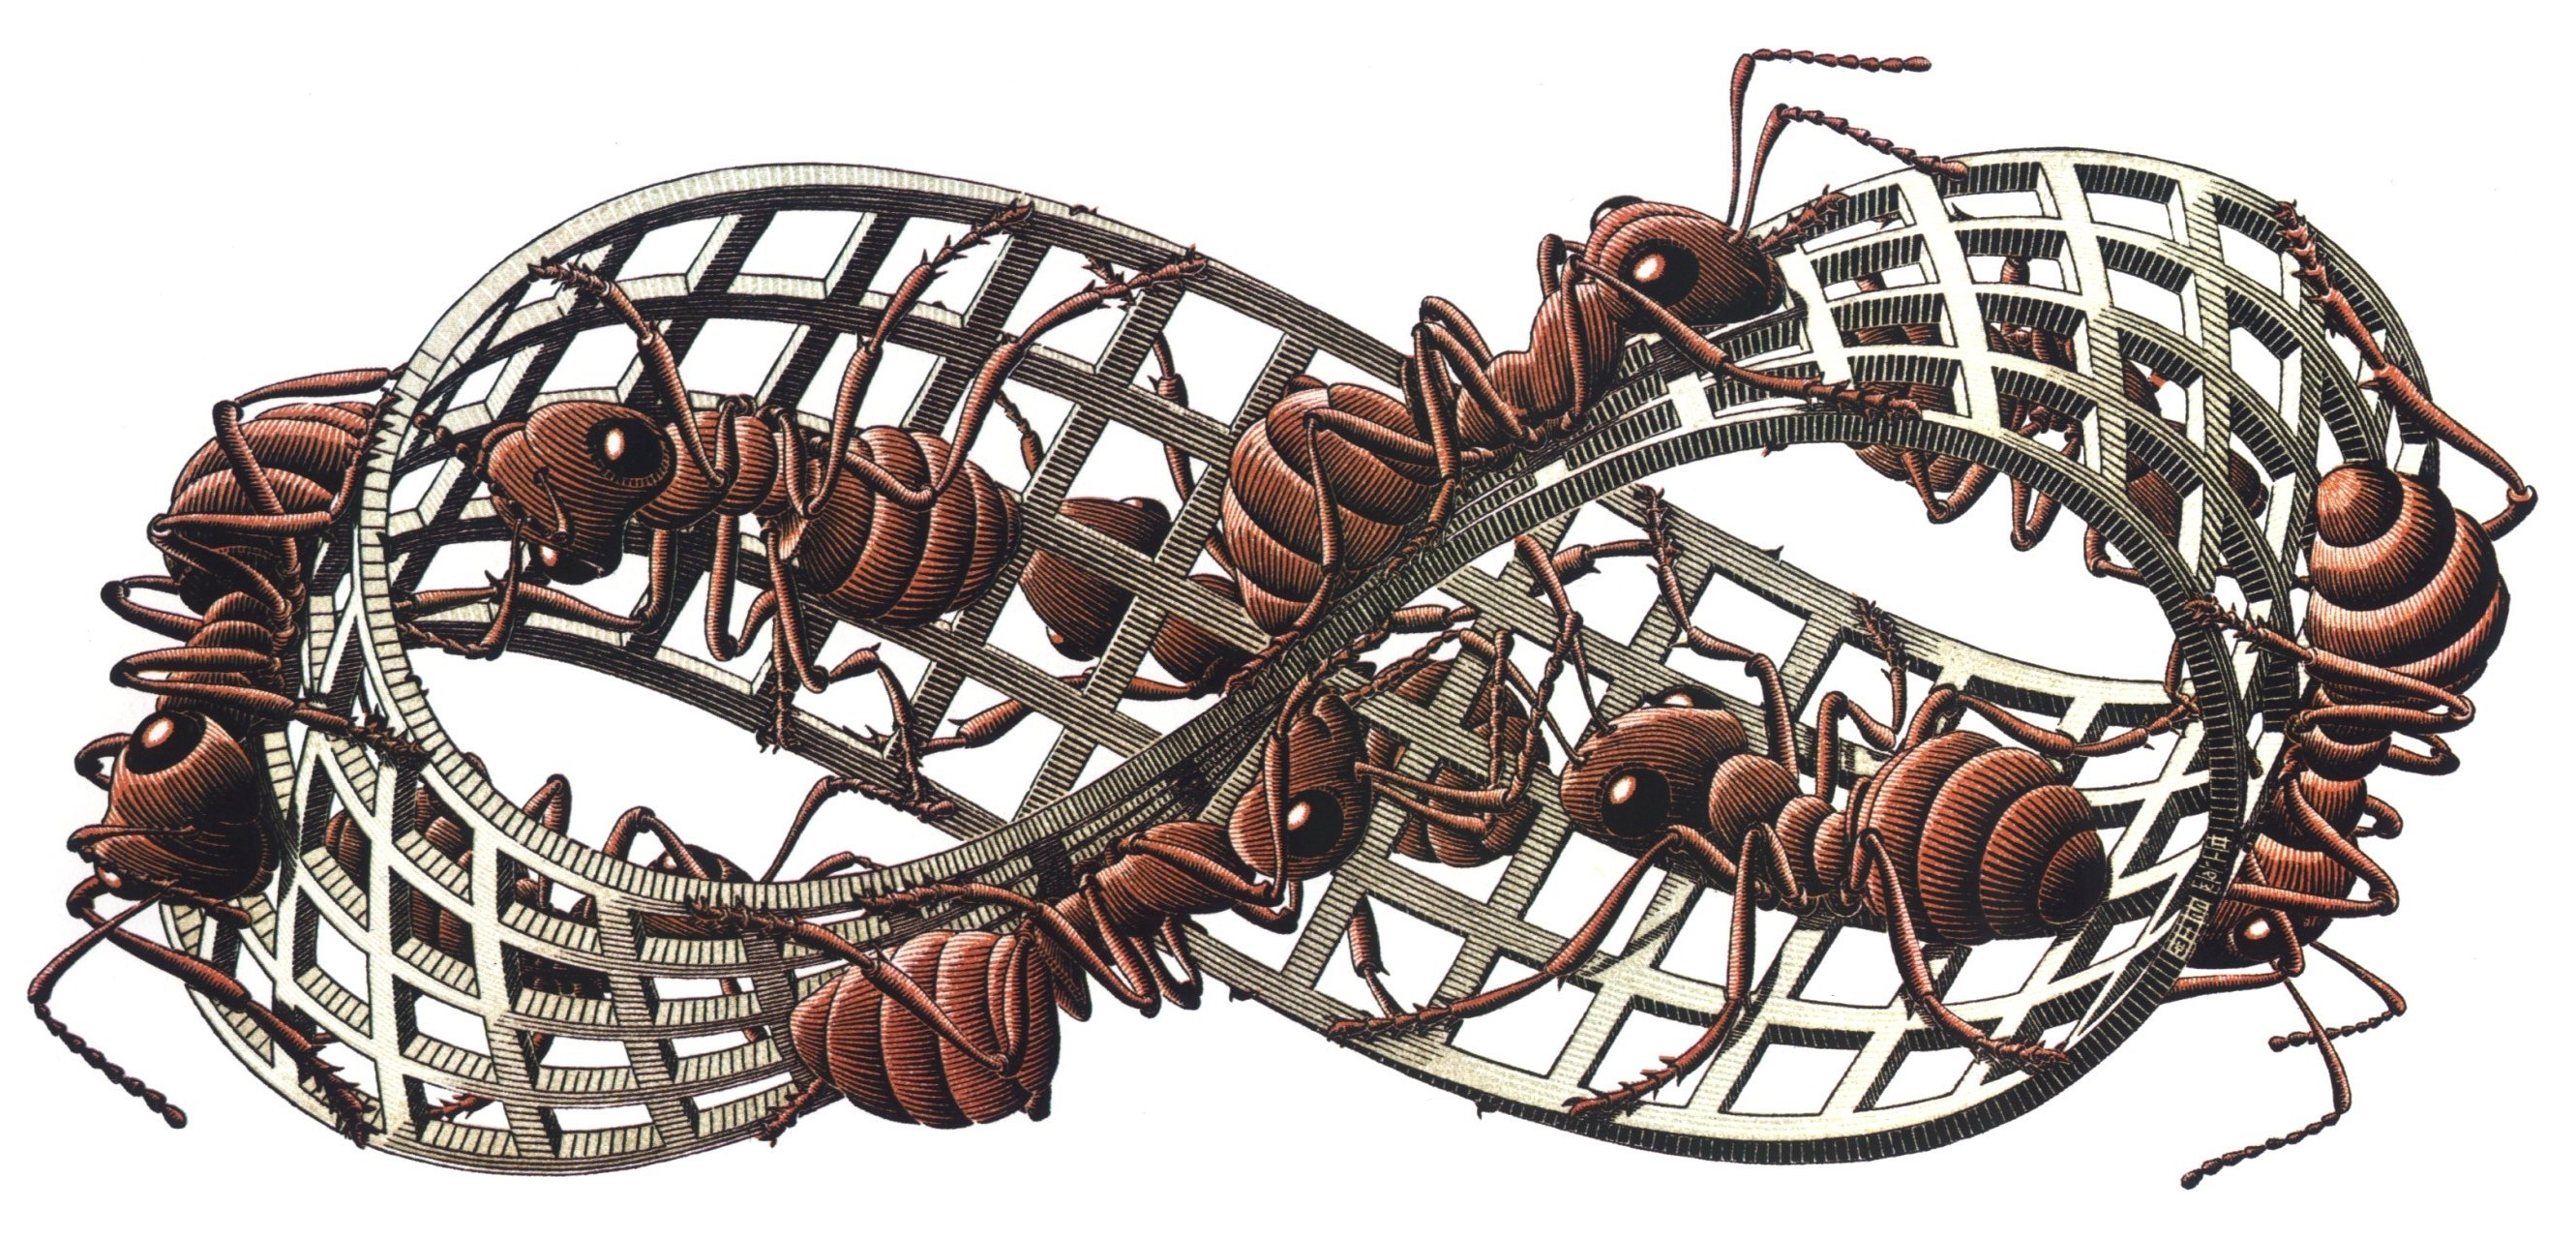
\includegraphics[width=\textwidth]{chapters/040-green/images/ants.jpg}
\caption{Krabbelt eine Ameise auf einer Seite eines Möbius-Bandes,
findet sie sich nach einem Umlauf auf der anderen Seite wieder, da
das Möbius-Band eine nicht orientierbare Mannigfaltigkeit ist.
Stich von M.~C.~Escher.
\label{buch:green:fig:ants}}
\end{figure}
%
Der Unterschied zwischen den beiden Mannigfaltigkeiten der Beispiele
\ref{buch:green:green:beispiel:band}
und
\ref{buch:green:green:beispiel:moebius}
ist, dass das Möbius-Band nicht orientierbar ist.
Lässt man eine Ameise wie in Abbildung~\ref{buch:green:fig:ants}
entlang dem Möbius-Band krabbeln, wird sie
sich nach einem Umlauf um das Band auf der anderen Seite des Bandes
wiederfinden.
Sie muss also nochmals einen weiteren Umlauf ausführen, um wieder
am Ausgangspunkt auf der gleichen Seite wie beim Start anzukommen.

\begin{definition}
\label{buch:green:def:orientierung}
Eine differenzierbare zweidimensionale Mannigfaltigkeit heisst 
\emph{orientierbar}, wenn es eine 2-Form gibt, die nirgends
\index{orientierbar}%
verschwindet.
\end{definition}

Die Konstruktion des Atlas in den Beispielen zeigt, wie eine
alternative Beschreibung einer orientierbaren Mannigfaltigkeit
möglich wird.
Für die orientierbare Mannigfaltigkeit wurde ein Atlas gefunden,
dessen Kartenwechsel alle positive Determinanten hatten.
Für das nicht orientierbare Möbius-Band war dies nicht möglich.

\begin{definition}[orientierbarer Atlas]
Ein \emph{orientierbarer Atlas} einer differenzierbaren Mannigfaltigkeit
\index{Atlas!orientierbar}%
ist ein Atlas, dessen Kartenwechsel alle positive Determinante haben.
\index{Kartenwechsel}%
\end{definition}

Man kann zeigen, dass diese beiden Definitionen gleichwertig sind.
Dies ist der Inhalt des folgenden Satzes, den wir aber nicht
beweisen werden.

\begin{satz}
Eine zweidimensionale Mannigfaltigkeit ist genau dann orientierbar,
wenn es einen orientierbaren Atlas gibt.
\end{satz}


